\documentclass[12pt,a4paper,utf8x]{report}

\usepackage[frenchb]{babel}
\usepackage[T1]{fontenc}
\usepackage[final]{pdfpages} 

% Pour pouvoir utiliser 
\usepackage{ucs}
\usepackage{graphicx}
\usepackage[utf8x]{inputenc}

% Pour avoir de belles url
\usepackage{url}

\usepackage {geometry}

% Pour mettre du code source
\usepackage {listings}
\usepackage{verbatim}
\usepackage{fancyvrb}
\usepackage{minted}

% Pour pouvoir passer en paysage
\usepackage{lscape}

% Pour pouvoir faire plusieurs colonnes
\usepackage {multicol}
\usepackage{pifont}

\usepackage{float}
\restylefloat{figure}

% Pour les entetes de page
%\usepackage{fancyheadings}
%\pagestyle{fancy}
%\renewcommand{\sectionmark}[1]{\markboth{#1}{}} 
%\renewcommand{\subsectionmark}[1]{\markright{#1}} 

% Pour l'interligne de 1.5
\usepackage {setspace}
% Pour les marges de la page
\geometry{a4paper, top=2.5cm, bottom=2.5cm, left=2.5cm, right=2.5cm, marginparwidth=1.2cm}

\parskip=5pt %% distance entre § (paragraphe)
\sloppy %% respecter toujours la marge de droite 

% Pour les pénalités :
\interfootnotelinepenalty=150 %note de bas de page
\widowpenalty=150 %% veuves et orphelines
\clubpenalty=150 

%Pour la longueur de l'indentation des paragraphes
\setlength{\parindent}{15mm}

%%%% debut macro pour enlever le nom chapitre %%%%
\makeatletter
\def\@makechapterhead#1{%
 % \vspace*{30\p@}%
  {\parindent \z@ \raggedright \normalfont
    \interlinepenalty\@M
    \ifnum \c@secnumdepth >\m@ne
        \Huge\bfseries \thechapter\quad
    \fi
    \Huge \bfseries #1\par\nobreak
    \vskip 20\p@
  }}

\def\@makeschapterhead#1{%
%  \vspace*{30\p@}%
  {\parindent \z@ \raggedright
    \normalfont
    \interlinepenalty\@M
    \Huge \bfseries  #1\par\nobreak
    \vskip 20\p@
  }}
\makeatother
%%%% fin macro %%%%

\lstset{
basicstyle=\footnotesize,
numbers=left,
numberstyle=\normalsize,
breaklines=true,  
numbersep=7pt,
frame=single, 
}

\fvset{
frame=single,
fontsize==\footnotesize , 
numbers=left,
}

%Couverture 

\begin{document}

\begin{titlepage}
\hfill
  \begin{center}
    \begin{minipage}[t]{12cm} 
    \huge \center Classification non supervisée de photos
    \huge \center Fouille d'images
    \huge \center Mars 2014
    \end{minipage}
  \end{center}
\vfill
\begin{figure}[!h]
      \centering            
      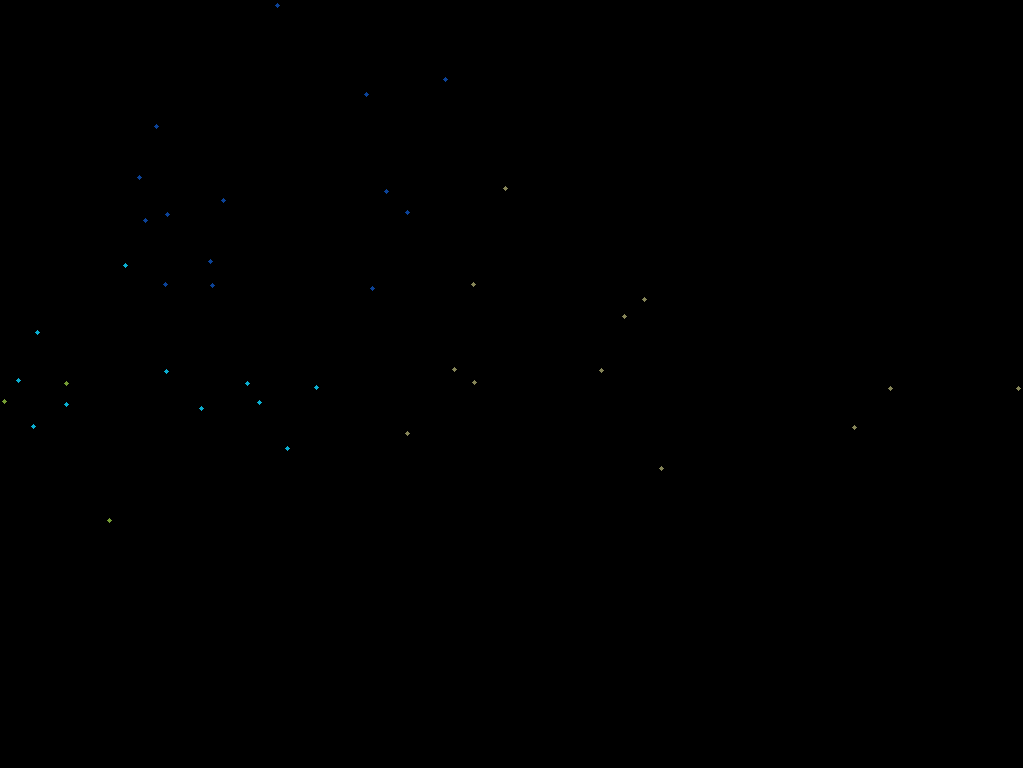
\includegraphics[width=0.8\textwidth]{ACP_SIFT.png} 
    \end{figure}
\begin{flushleft}
\begin{minipage}[t]{5cm}
Master 2 VIP, \\ Aurélien Cavelan et Jérôme Richard
\end{minipage}
\end{flushleft}

\end{titlepage}
%\clearpage
\tableofcontents

\chapter{Objectifs}

L'objectif de ce mini projet consiste à développer un système de classification automatique non supervisée de photos. Le système dispose initialement de photos annotées en cinq classes (que vous découvrirez aisément), fournies par l'enseignant, et comportant quelques pièges. Chaque photo se rattache à une seule classe. A partir de cet ensemble de photos annotées, le système doit extraire des descripteurs et proposer une classification non supervisée des images (clustering).


\chapter{Choix Logiciels}

\section{Approche}
    Nous avons envisagés plusieurs outils pour réaliser ce projet, parmis lesquels :

    \begin{itemize}
        \item Matlab
        \item C++ - OpenCV
        \item Python - Scikit / Skimage
        \item Python - OpenCV
    \end{itemize}

    Matlab n'est pas assez performant et ne permet pas de répondre à tous nos besoins. Il n'est pas assez bas-niveaux et ne permet pas de développer un réel outils.

    Python est un langage très simple et il existe un kit de développement performant (binding C) disposant d'outils pour la classification, l'apprentissage et la manipulation d'images. Le manque de documentation et d'exemples nous a pousser à regarder du côté d'OpenCV.

    Le couple C++ OpenCV est probablement l'un des choix les plus courant pour la tâche qui nous est donnée. OpenCV est une bibliothèque très performante, bien qu'elle soit moins accessible que les options précédentes. On trouve néanmoins de nombreux exemples de codes utilisant OpenCV, et notamment pour lire des images, appliquer des filtres, extraire des descripteurs, ou encore utiliser l'algorithme des K-Moyennes ou la classification hiérarchique. C'est donc sur cette base que nous avons décidé de partir.

    Dans un premier temps nous avons décidé d'implémenté un descripteur "moyenne de niveau de gris" car c'est un descripteur a une seule dimension et il est donc facile de vérifier les résultats de l'algorithmes K-Moyennes. Nous avons également créé des jeux de données plus simples disponibles dans data2, data3 et data4 afin de comparer plus simplement les descripteurs.


\section{Apprentissage}
    TODO

\section{Architecture}
    Le code est entièrement écrit en C++ et utilise la bibliothèque OpenCV. Un Makefile à la racine permet de compiler les différents algorithmes de classifications.

    Le programme prend en entré un fichier .csv décrivant les images à utiliser et les classes auxquelles elles appartiennent. Le programme se sert d'une base d'images afin de déterminer les centres, soit par l'algorithme des K-Moyennes, soit par la classification hiérarchique (dendrogramme). Le programme classifie ensuite la totalité des images et affiche les résultats en mode texte, ainsi que l'indice de Rand et l'ACP sur deux dimensions.

    Le code du programme est peut fonctionner avec n'importe quel type de descripteurs et se trouve dans le fichier src/main.cpp. Les descripteurs implémentés se trouvent dans le fichier src/descriptors.cpp. Un descripteur est défini comme étant un ensemble de nombre floatants, typiquement 1 pour le descripteur "moyenne de niveau de gris" et 128 pour le descripteur "SURF".

    La répartitions des images est également afficher lors de l'exécution du programme. Il est aussi possible d'exporter la position des centres dans fichier.

    Un certain nombre de données sont sauvegardés au format yml lors de l'exécution, tels que les descripteurs de SURF et de SIFT ainsi que le dicionnaire (Bag of Words) associé. Ils peuvent ainsi être réutilisé par OpenCV pour éviter de reclaculer l'ensemble des descripteurs, ce qui peut prendre plus d'une minute.


\chapter{Descripteurs}
    Nous avons implémenté plusieurs descripteurs, certains très simple (et peu efficaces), et d'autres plus complexes mais aussi plus performants. Nous avons comparés ces descripteurs selon plusieurs critères, en comparant les résultats obtenus avec l'Algorithme des K-Moyennes et la classification hiérarchique, mais aussi leur résistances à diverses transformations ou encore leur performance.

    \section{Descripturs 1D}
        [Moyenne en niveau de gris]
        [variance]

    \section{Moments de Hu}
        [Fonctionne pas sans contours]

    \section{SIFT / SURF}
        [Décrire le principe de fonctionnement]

      SURF / SIFT :
      - stockage dans des fichiers
      - performance
      - décrire le processus

==> Mettre ici les screens ACP


\chapter{Synthèse}

Tableau synthétique en latex


\chapter{Conclusion}
    [SIFT is better than SURF]
    [but SURF is FASTER than SIFT]
    [Les images sont pourries]
    [C'est super dur de classifier correctement des images et ya sans cesse de nouveaux descripteurs qui font l'objets d'articles, c'est pas pour rien.]

  
\end{document}

    
